% SC1004 Chapter 6: Orthogonality & Least Squares (0->100 ground-up)
\chapter{Orthogonality and Least Squares}
\label{ch:orthogonality}

\begin{quote}
\emph{``Orthogonality is geometry's way of saying `no shadow'.''} When a system $A\mathbf{x}=\mathbf{b}$ has no solution, the closest we can do is the shadow of $\mathbf{b}$ on the column space --- that shadow solves the least-squares problem.
\end{quote}

\noindent\fbox{\parbox{\dimexpr\linewidth-2\fboxsep-2\fboxrule}{%
\textbf{From zero: right angles before residuals.} We generalise $\mathbf{u}\cdot\mathbf{v}=0$ from $\mathbb{R}^2$ to $\mathbb{R}^n$, build orthogonal projections, then solve $A\mathbf{x}\approx\mathbf{b}$ when equality is impossible --- the workhorse of regression and data fitting.}}
\vspace{0.4em}

\section*{Learning Outcomes}
After this chapter you will be able to:
\begin{enumerate}[label=(L\arabic*)]
    \item test orthogonality and orthonormality of sets;
    \item compute orthogonal projections onto subspaces;
    \item run Gram--Schmidt to build orthonormal bases and $QR$;
    \item formulate and solve least-squares via normal equations and $QR$;
    \item apply least squares to line fitting and explain residuals.
\end{enumerate}

% ============================================================
\section{Orthogonality in \texorpdfstring{$\mathbb{R}^n$}{Rn}}
\label{sec:ortho-def}
Recall $\mathbf{u}\perp\mathbf{v}\iff\mathbf{u}\cdot\mathbf{v}=0$ (Ch.~1). A set $\{\mathbf{q}_1,\dots,\mathbf{q}_k\}$ is \emph{orthogonal} if each pair is orthogonal; \emph{orthonormal} if in addition $\|\mathbf{q}_i\|=1$. Orthonormal sets are automatically independent --- no one can be built from perpendicular directions.

\begin{figure}[h]
\centering
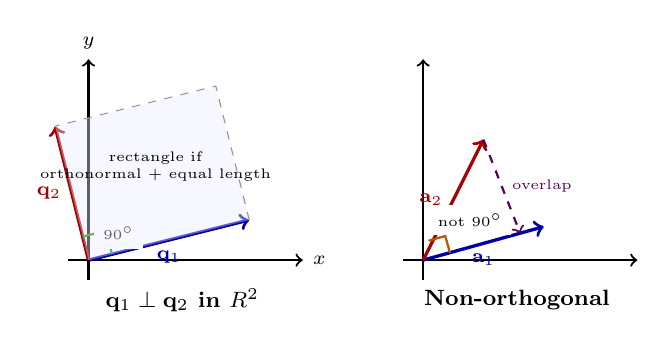
\begin{tikzpicture}[scale=0.85,every node/.style={font=\scriptsize}]
  \draw[->,thick] (-0.3,0)--(3.2,0) node[right] {$x$};
  \draw[->,thick] (0,-0.3)--(0,3.0) node[above] {$y$};
  \draw[->,very thick,blue!65!black] (0,0)--(2.4,0.6) node[midway,below] {$\mathbf{q}_1$};
  \draw[->,very thick,red!65!black] (0,0)--(-0.5,2.0) node[midway,left] {$\mathbf{q}_2$};
  \draw[thick,green!60!black] (0.35,0.09)--(0.26,0.44)--(-0.09,0.35);
  \node[font=\tiny,fill=white] at (0.45,0.4) {$90^\circ$};
  \draw[dashed,gray] (2.4,0.6)--(1.9,2.6)--(-0.5,2.0);
  \fill[blue!8,opacity=0.4] (0,0)--(2.4,0.6)--(1.9,2.6)--(-0.5,2.0)--cycle;
  \node[font=\tiny,align=center] at (1.0,1.4) {rectangle if\\orthonormal + equal length};
  \node[font=\footnotesize\bfseries] at (1.4,-0.6) {$\mathbf{q}_1\perp\mathbf{q}_2$ in $\mathbb{R}^2$};

  \begin{scope}[xshift=5.0cm]
    \draw[->,thick] (-0.3,0)--(3.2,0); \draw[->,thick] (0,-0.3)--(0,3.0);
    \draw[->,very thick,blue!65!black] (0,0)--(1.8,0.5) node[midway,below] {$\mathbf{a}_1$};
    \draw[->,very thick,red!65!black] (0,0)--(0.9,1.8) node[midway,left] {$\mathbf{a}_2$};
    \draw[thick,orange!70!black] (0.4,0.11)--(0.33,0.36)--(0.08,0.29);
    \node[font=\tiny,fill=white] at (0.7,0.6) {not $90^\circ$};
    \draw[->,thick,violet!70!black,dashed] (0.9,1.8)--(1.45,0.4) node[midway,right,font=\tiny] {overlap};
    \node[font=\footnotesize\bfseries] at (1.4,-0.6) {Non-orthogonal};
  \end{scope}
\end{tikzpicture}
\caption{Left: orthogonal vectors meet at $90^\circ$; orthonormal adds unit length. Right: general non-orthogonal pair (Gram--Schmidt will fix this).}
\label{fig:orthogonality}
\end{figure}

If $Q=[\mathbf{q}_1\cdots\mathbf{q}_k]$ has orthonormal columns, then $Q^TQ=I_k$ --- columns are perfectly conditioned; $Q$ preserves lengths: $\|Q\mathbf{x}\|=\|\mathbf{x}\|$.

\section{Projections onto Subspaces}
\label{sec:projections}
Let $W=\operatorname{span}\{\mathbf{a}_1,\dots,\mathbf{a}_k\}\subseteq\mathbb{R}^n$. For $\mathbf{b}\in\mathbb{R}^n$, the \emph{projection} $\hat{\mathbf{b}}=\operatorname{proj}_W\mathbf{b}$ is the unique $\mathbf{w}\in W$ closest to $\mathbf{b}$; the residual $\mathbf{b}-\hat{\mathbf{b}}$ is orthogonal to $W$.

When $W$ has orthonormal basis $Q$,
\[
  \operatorname{proj}_W\mathbf{b}=QQ^T\mathbf{b}=\sum_{i=1}^{k}(\mathbf{q}_i^T\mathbf{b})\,\mathbf{q}_i.
\]
In general with $A=[\mathbf{a}_1\cdots\mathbf{a}_k]$ (full column rank),
\[
  \operatorname{proj}_W\mathbf{b}=A(A^TA)^{-1}A^T\mathbf{b}.
\]
The matrix $P=A(A^TA)^{-1}A^T$ satisfies $P^2=P$, $P^T=P$ --- the orthogonal projector onto $\mathcal{C}(A)$.

\begin{figure}[h]
\centering
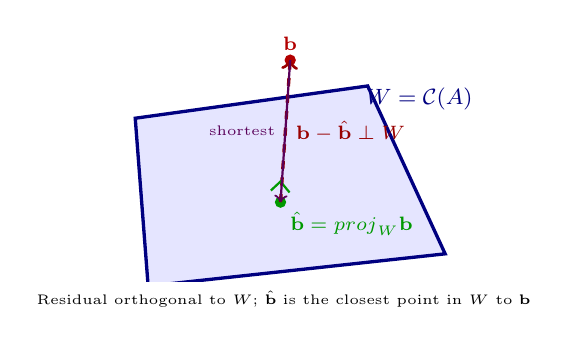
\begin{tikzpicture}[scale=0.82,every node/.style={font=\scriptsize}]
  \fill[blue!10] (-1.2,-0.3)--(3.4,0.2)--(2.2,2.8)--(-1.4,2.3)--cycle;
  \draw[very thick,blue!50!black] (-1.2,-0.3)--(3.4,0.2)--(2.2,2.8)--(-1.4,2.3)--cycle;
  \node[font=\footnotesize\bfseries,blue!50!black] at (3.0,2.6) {$W=\mathcal{C}(A)$};
  \fill[red!70!black] (1.0,3.2) circle (2.5pt) node[above] {$\mathbf{b}$};
  \fill[green!60!black] (0.85,1.0) circle (2.5pt) node[below right] {$\hat{\mathbf{b}}=\operatorname{proj}_W\mathbf{b}$};
  \draw[->,very thick,red!60!black,dashed] (0.85,1.0)--(1.0,3.2) node[midway,right] {$\mathbf{b}-\hat{\mathbf{b}}\perp W$};
  \draw[thick,green!60!black] (0.70,1.18)--(0.85,1.32)--(0.99,1.15);
  \draw[->,thick,violet!70!black] (1.0,3.2)--(0.85,1.0) node[midway,left,font=\tiny] {shortest};
  \node[font=\tiny,fill=white] at (0.9,-0.5) {Residual orthogonal to $W$; $\hat{\mathbf{b}}$ is the closest point in $W$ to $\mathbf{b}$};
\end{tikzpicture}
\caption{Orthogonal projection: $\hat{\mathbf{b}}$ is the closest point in $W$ to $\mathbf{b}$; the error $\mathbf{b}-\hat{\mathbf{b}}$ is perpendicular to $W$.}
\label{fig:projection-subspace}
\end{figure}

\section{Gram--Schmidt and QR}
\label{sec:gram-schmidt}
Gram--Schmidt turns any independent $\mathbf{a}_1,\dots,\mathbf{a}_k$ into orthonormal $\mathbf{q}_1,\dots,\mathbf{q}_k$ spanning the same nested subspaces:

\begin{align}
  \mathbf{u}_1&=\mathbf{a}_1,\quad \mathbf{q}_1=\mathbf{u}_1/\|\mathbf{u}_1\|,\\
  \mathbf{u}_2&=\mathbf{a}_2-(\mathbf{q}_1^T\mathbf{a}_2)\mathbf{q}_1,\quad \mathbf{q}_2=\mathbf{u}_2/\|\mathbf{u}_2\|,\\
  &\ \vdots\\
  \mathbf{u}_k&=\mathbf{a}_k-\sum_{i<k}(\mathbf{q}_i^T\mathbf{a}_k)\mathbf{q}_i.
\end{align}
Each step subtracts the shadows already accounted for. With $A=QR$ ($Q$ orthonormal columns, $R$ upper-triangular), $R=Q^TA$ records the coefficients.

\begin{figure}[h]
\centering
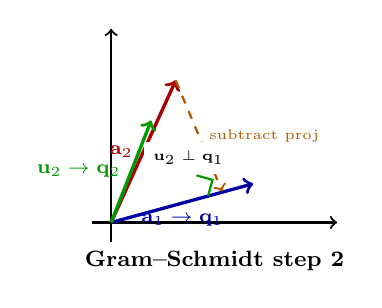
\begin{tikzpicture}[scale=0.82,every node/.style={font=\scriptsize}]
  \draw[->,thick] (-0.3,0)--(3.5,0); \draw[->,thick] (0,-0.3)--(0,3.0);
  \draw[->,very thick,blue!65!black] (0,0)--(2.2,0.6) node[midway,below] {$\mathbf{a}_1\to\mathbf{q}_1$};
  \draw[->,very thick,red!65!black] (0,0)--(1.0,2.2) node[midway,left] {$\mathbf{a}_2$};
  \draw[->,thick,orange!70!black,dashed] (1.0,2.2)--(1.72,0.48) node[midway,right,font=\tiny] {subtract proj};
  \draw[->,very thick,green!60!black] (0,0)--(0.62,1.58) node[midway,left] {$\mathbf{u}_2\to\mathbf{q}_2$};
  \draw[thick,green!60!black] (1.50,0.41)--(1.57,0.66)--(1.32,0.73);
  \node[font=\tiny,fill=white] at (1.2,1.0) {$\mathbf{u}_2\perp\mathbf{q}_1$};
  \node[font=\footnotesize\bfseries] at (1.6,-0.6) {Gram--Schmidt step 2};
\end{tikzpicture}
\caption{Gram--Schmidt: subtract from $\mathbf{a}_2$ its projection on $\mathbf{q}_1$; what remains is orthogonal to $\mathbf{q}_1$. Normalise to get $\mathbf{q}_2$.}
\label{fig:gram-schmidt}
\end{figure}

\begin{example}[QR by hand ($2\times2$)]
$A=\begin{bmatrix}1&1\\1&0\\0&1\end{bmatrix}$ ($3\times2$): $\mathbf{q}_1=[1,1,0]^T/\sqrt2$, $\mathbf{u}_2=[1,0,1]^T-(\mathbf{q}_1^T[1,0,1]^T)\mathbf{q}_1=[1/2,-1/2,1]^T$, $\mathbf{q}_2=\mathbf{u}_2/\|\mathbf{u}_2\|$. Then $R=Q^TA$ is $2\times2$ upper-triangular.
\end{example}

\section{Least Squares}
\label{sec:least-squares}
When $A\mathbf{x}=\mathbf{b}$ has no solution ($\mathbf{b}\notin\mathcal{C}(A)$), minimise the squared error:
\[
  \min_{\mathbf{x}}\|A\mathbf{x}-\mathbf{b}\|^2.
\]
The minimiser $\hat{\mathbf{x}}$ makes $A\hat{\mathbf{x}}=\operatorname{proj}_{\mathcal{C}(A)}\mathbf{b}$, so the residual is orthogonal to $\mathcal{C}(A)$: $A^T(\mathbf{b}-A\hat{\mathbf{x}})=\mathbf{0}$.

\begin{theorem}[Normal equations]
$\hat{\mathbf{x}}$ is a least-squares solution iff
\[
  A^TA\hat{\mathbf{x}}=A^T\mathbf{b}.
\]
If $A$ has independent columns, $A^TA$ is invertible and $\hat{\mathbf{x}}=(A^TA)^{-1}A^T\mathbf{b}$ is unique. With $A=QR$, $\hat{\mathbf{x}}=R^{-1}Q^T\mathbf{b}$ (more stable).
\end{theorem}

\begin{example}[Line fitting]
Fit $y=c+dt$ through $(t_i,y_i)$: $A=\begin{bmatrix}1&t_1\\\vdots&\vdots\\1&t_m\end{bmatrix}$, $\mathbf{x}=[c,d]^T$. Then $A^TA=\begin{bmatrix}m&\sum t_i\\\sum t_i&\sum t_i^2\end{bmatrix}$, $A^T\mathbf{b}=[\sum y_i,\sum t_iy_i]^T$. Solving gives the regression line; $\|\mathbf{b}-A\hat{\mathbf{x}}\|$ is the residual.
\begin{lstlisting}[language=Python]
import numpy as np
t = np.array([0.,1.,2.,3.])
y = np.array([1.1,1.9,3.2,3.8])
A = np.column_stack([np.ones_like(t), t])
x_hat, residuals, rank, s = np.linalg.lstsq(A, y, rcond=None)
print(x_hat)  # [c, d] intercept + slope
# Compare with normal equations:
print(np.linalg.solve(A.T@A, A.T@y))
\end{lstlisting}
\end{example}

% ============================================================

% --- Additional depth: Orthogonal complements and best approximation ---
\section{Orthogonal Complements and the Four Subspaces}
\label{sec:ortho-complement}
For $W\subseteq\mathbb{R}^n$, $W^\perp=\{\mathbf{x}:\mathbf{x}\perp\mathbf{w}\;\forall\mathbf{w}\in W\}$ is a subspace with $\dim W+\dim W^\perp=n$ and $(W^\perp)^\perp=W$. Fundamental theorem:
\[
  \mathcal{C}(A)^\perp=\mathcal{N}(A^T),\qquad \mathcal{C}(A^T)^\perp=\mathcal{N}(A).
\]
So $\mathbb{R}^n=\mathcal{C}(A^T)\oplus\mathcal{N}(A)$ and $\mathbb{R}^m=\mathcal{C}(A)\oplus\mathcal{N}(A^T)$ as orthogonal direct sums. The least-squares residual lives in $\mathcal{N}(A^T)$.

\section{Best Approximation and the Projection Theorem}
\label{sec:best-approx}
\begin{theorem}[Projection theorem]
Let $W\subseteq\mathbb{R}^n$ be a subspace. For any $\mathbf{b}$, there is a unique $\hat{\mathbf{b}}\in W$ minimising $\|\mathbf{b}-\hat{\mathbf{b}}\|$, namely $\hat{\mathbf{b}}=\operatorname{proj}_W\mathbf{b}$. Moreover $\mathbf{b}-\hat{\mathbf{b}}\in W^\perp$.
\end{theorem}
This underpins all of least squares: $A\hat{\mathbf{x}}$ is the best approximation to $\mathbf{b}$ from $\mathcal{C}(A)$. Error $\|\mathbf{b}-A\hat{\mathbf{x}}\|$ is the distance from $\mathbf{b}$ to the subspace.

\section{Numerical Stability: QR vs.\ Normal Equations}
\label{sec:stability}
Forming $A^TA$ squares the condition number $\kappa(A^TA)=\kappa(A)^2$, so normal equations lose half the digits when $A$ is ill-conditioned. $QR$ avoids this: $Q$ is perfectly conditioned ($\kappa(Q)=1$), so solving $R\hat{\mathbf{x}}=Q^T\mathbf{b}$ is stable. Modified Gram--Schmidt and Householder $QR$ are preferred; NumPy's \texttt{lstsq} uses SVD/Householder internally.



\begin{example}[Polynomial least squares]
Fit a parabola $y=c_0+c_1t+c_2t^2$ to $m$ points: $A$ is $m\times3$ Vandermonde $[1\ t_i\ t_i^2]$. Columns become nearly dependent for large $t_i$ (ill-conditioned); centering $t_i$ or using orthogonal polynomials (Legendre) fixes this. \texttt{np.polyfit} does a scaled $QR$ internally for this reason.
\end{example}

\begin{remark}[When $A^TA$ is singular]
If $A$ has dependent columns, $A^TA$ singular and normal equations have infinitely many solutions. The minimal-norm least-squares solution is $A^\dagger\mathbf{b}$ where $A^\dagger=V\Sigma^\dagger U^T$ is the pseudoinverse (SVD, Ch.~8). NumPy's \texttt{lstsq} returns this by default.
\end{remark}



\begin{remark}[Geometric meaning of $Q^TQ=I$]
Columns $\mathbf{q}_i$ orthonormal $\iff$ $Q$ is an isometry on its column space: angles and lengths preserved. In graphics, $Q$ is a rotation/reflection; in data science, $Q$ from $QR$ is the ``well-conditioned'' part of $A$. Never form $Q$ explicitly when $m\gg n$ --- Householder applies $Q^T\mathbf{b}$ implicitly in $O(mn)$.
\end{remark}


\section{Chapter Notes}
Least squares (Legendre, Gauss, 1805--1809) predates matrices; Gauss used it to predict Ceres' orbit. $QR$ via Gram--Schmidt or Householder reflections is the stable solver (LAPACK's \texttt{gels}); forming $A^TA$ squares the condition number and is avoided for ill-conditioned $A$.

% ============================================================
\section{Exercises}
\label{sec:ch06-exercises}
\begin{enumerate}[label=E6.\arabic*, leftmargin=*, itemsep=0.8em]
\item \textbf{Orthonormal check.} Is $Q=\frac12\begin{bmatrix}1&1&1&1\\1&-1&1&-1\\1&1&-1&-1\\1&-1&-1&1\end{bmatrix}$ orthogonal ($Q^TQ=I$)? What is $Q\mathbf{x}$ geometrically?
\item \textbf{Gram--Schmidt.} Apply Gram--Schmidt to $\mathbf{a}_1=[1,1,0]^T$, $\mathbf{a}_2=[1,0,1]^T$, $\mathbf{a}_3=[0,1,1]^T$ in $\mathbb{R}^3$. Write $A=QR$ and verify $Q^TQ=I$, $A=QR$.
\item \textbf{Projection matrix.} For $A=[1,1,1]^T$ (span of all-ones vector in $\mathbb{R}^3$), compute $P=A(A^TA)^{-1}A^T$. Show $P^2=P$, $P^T=P$, and $P\mathbf{b}$ is the mean of entries times $\mathbf{1}$.
\item \textbf{Least squares.} Fit $y=c+dt$ to $(0,1),(1,2),(2,2),(3,4)$ via normal equations. Compute $\hat{\mathbf{x}}$ and $\|\mathbf{b}-A\hat{\mathbf{x}}\|$. Verify $A^T(\mathbf{b}-A\hat{\mathbf{x}})=\mathbf{0}$.
\item \textbf{Coding.} Generate $m=100$ noisy points $y=2+3t+\mathcal{N}(0,0.5)$, $t\in[0,5]$. Solve least squares via (a) normal equations and (b) \texttt{np.linalg.lstsq} ($QR$). Compare $\hat{\mathbf{x}}$ and residuals; which is more stable if you add an outlier?
\end{enumerate}
% End of Chapter 6
